\section{Decision tree}

%%%%%%%%%%%%%%%%%%%%%%%%%%%%%%%
\subsection{Main idea}
The Decision Tree is a non-parametric supervised learning method used for classification and regression.
It predicts the response with a set of if-then-else decision rules derived from the data.
The deeper the tree, the more complex the decision rules and the closer the model fits the data.
The Decision Tree builds classification or regression models in form of a tree structure.
Each node in the tree further splits the feature space into smaller and smaller subsets, 
while at the same time an associated Decision Tree is incrementally developed.
The final result is a tree with decision nodes and terminal nodes. 
A decision node has two or more branches.
Leaf nodes represent the actual classification or decision. 
The topmost decision node in a tree that corresponds to the best predictor is called the root node.
Decision trees can handle both categorical and numerical data.

An example of such a tree is depicted below in figure \ref{fig:decision_tree_example}.

\begin{figure}[H]
    \captionsetup{format=plain}
    \makebox[\textwidth]{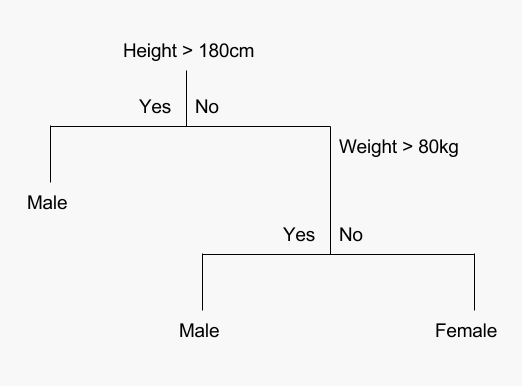
\includegraphics[width=100mm]{decision_tree_example.png}}
    \caption{Given a data set with two features height and weight, and gender as the target variable, 
             this example tree stratifies the two-dimensional feature space into three distinct subsets each 
             represented by the terminal nodes at the bottom.
             The stratification occurs at the two deciding nodes depending either on whether its height is above 180 cm 
             and its weight is above 80kg.
             }
    \label{fig:decision_tree_example}
\end{figure}
%%%%%%%%%%%%%%%%%%%%%%%%%%%%%%%
\subsection{Tree Building Process}
This chapter describes the CART algorithm for tree building as specified in \cite{breiman1984classification}.
The basic idea of tree growth is to choose a split among all the possible splits at each node
such that the resulting child nodes are the “purest”. In this algorithm, only univariate splits are
considered. That is, each split depends on the value of only one predictor variable. All
possible splits consist of possible splits of each predictor.

A tree is grown starting from the root node by repeatedly using the following steps on each
node in the following algorithm:

\begin{algorithm}[H]
    \caption{Binary Splitting \cite{breiman1984classification}}
    \label{alg:binary_splitting}
    \SetAlgoLined
    \begin{itemize}
        \item[(i)] \textbf{Find best split \(s\) for each feature \(X_{m}\):}
        For each feature \(X_{m}\), there exist \(K-1\)-many potiential splits, 
        whereas \(K\) is the number of different values for the respective feature.
        Evaluate each value \(X_{m,i}\) at the current node \(t\) as a 
        candidate split point (for \(x \in X_{m}\), if \(x \leq X_{m,i}=s\),
        then \(x\) goes to left child node \(t_{L}\) else to right child node \(t_{R}\)).
        The best split point is the one that maximize the splitting criterion \(\ \Delta i(s,t) \) the most when the node is split according to it.
        The different splitting criteria will be covered in the next chapter.

        \item[(ii)] \textbf{Find the node’s best split:} Among the best splits for each feature from Step (i) find the 
        one \(s^{*}\), which maximizes the splitting criterion \(\Delta i(s,t)\).

        \item[(iii)] \textbf{Satisfy stopping criterion:} Split the node \(t\) using best node split \(s^{*}\) from Step (ii) 
        and repeat from Step (i) until stopping criterion is satisfied. 
    \end{itemize}
    \end{algorithm}


%%%%%%%%%%%%%%%%%%%%%%%%%%%%%%%
\subsubsection{Splitting criteria}
Since we are only concerned with classification, \(Y\) is categorical. The original CART algorithm uses Gini and Towing as 
purity measures for the splitting criterion \cite{breiman1984classification}. 
However, implementations of the algorithm such as Python's sklearn package \cite{scikit2011learn} also contain entropy and misclassification rate as measures of impurity.

For a given learning sample \( D = {(x_{1},y_{1}), (x_{2}, y_{2}), ... , (x_{N}, y_{N})} \) 
for a \(C\) class problem, let \(N_{c}\) be the number of instances \( \{x,y\}  \)
belonging to class \(c\).

In node \(t\), let \(N(t)\) be the total number of instances with \( \{x,y\} \in t \) 
and \( N_{c}(t) \) the number of class \(c\) instances in \(t\). 
The proportion of the instances belonging to class \(c\) in the sample \(D\) falling into \(t\) 
equals \( N_{c}(t) / N_{j} \).
The given set of priors \( \pi(c) \) specify the probability that an instance belongs to class \(c\).

At node \(t\), let the probabilities \(p(c,t)\) be estimated by 

\begin{equation}
    p(c,t) = \frac{ \pi(c)N_{c}(t) }{ N_{c} }.
\end{equation}

This represents the probability that an instance will both be in class \(c\) and fall into node \(t\).
Therefore, the estimate for the probability that any instance falls into node \(t\) is defined by

\begin{equation}
    p(t) = \sum_{c \in C} p(c,t),
\end{equation}

The estimate \( p(t) \) for the probability that an instance belongs to class \(c\) given that it falls into node \(t\) is defined by

\begin{equation}
    p(c|t) = \frac{ p(c,t)}{ p(t) } = \frac{ p(c,t) }{ \sum_{c \in C} p(c,t) }.
\end{equation}

Further, it holds that the conditional probability \(p(c|t)\) must satisfy

\begin{equation}
    \sum_{c \in C} p(c|t)  = 1
\end{equation}

Let \(i(t)\) be an impurity measure evaluated at note \(t\). 
Then, the decrease of impurity (i.e. the splitting criterion) is defined as

\begin{equation}
    \Delta i(s,t) = i(t) - p_{L} i(t_{L}) - p_{R} i(t_{R}),
\end{equation}

where \(p_{L}\) and \(p_{R}\) are probabilities of sending a case to the left child node \(t_{L}\) and to the
right child node \(t_{R}\) respectively. 
They are defined as \( p_{L} = p(t_{L}) / p(t) \) and \( p_{R} = p(t_{R}) / p(t) \).

As already stated above, the goal is to maximize \(\Delta i(s,t)\).
In the following, different measures for impurity will be presented.

\textbf{Gini Measure}

The Gini impurity measure is defined as 

\begin{equation}
    i(t) = \sum_{c \in C} p(c|t) (1 - p(c|t)) = 1 - \sum_{c \in C} p_{c}^{2}
\end{equation}

The intuition behind this measure is to assign nodes 
for which its probabilities are more skewed towards a particular group for a higher value.
Conversely, if a node has a more balanced distribution, then \(i(t)\) will turn out to be lower.
For example, in the case of \( |C|=2 \), \(i(t)\) will be maximized by \( p(c|t) = 0.5 \) for \( c \in C \).


\textbf{Information Entropy}

The Entropy measure from information theory is defined as

\begin{equation}
    i(t) = \sum_{c \in C} p(c|t) log(p(c|t)),
\end{equation}

which measures the average rate at which information is produced by a stochastic source of data.
Thus, it can also be used for measuring impurity.

\textbf{Rate of Misclassification}

The rate of misclassification is defined as 
\begin{equation}
    i(t) = 1 - \max_{c \in C} p(c|t) .
\end{equation}
which measures the proportion of instances node \(t\) not belonging to the dominant group in \(t\).


%%%%%%%%%%%%%%%%%%%%%%%%%%%%%%%%%%%%%
\subsubsection{Bias-variance trade-off}
We can measure the performance of a Decision Tree by assessing its fit to the data. 
The generalization error is a widely used concept for evaluating the fit \cite{breiman2001random}.
In this paper, we use generalization error to compare methods and adjust parameters to improve methods. 
Under certain assumptions, we can decompose the generalization error into three main components:
the Bayes Error, the squared bias ($bias^2$) and the variance. 
We will explain the mathematical aspects of the generalization error in the following chapters. 
For now, we only need to mention the Bayes Error is irreducible and independent of the classifier, 
and there is a trade-off between $bias^2$ and variance. Since Decision Trees suffer from high variance and 
decreasing variance causes $bias^2$ to increase \cite{geman1992neural}, we need methods to bypass this trade-off. 
These methods include Bagging, Boosting and Random Forest 
which exploits mathematical properties to decrease variance without increasing $bias^2$. 
We will explain bagging briefly, exhibit mathematical dynamics of Random Forest and 
use Boosting in the application section.


\subsection{Bagging}
Decision Tree belongs to methods that are sensitive to the specific data on which they are trained \cite{friedman2001elements}. 
In other words, Decision Tree estimates are susceptible to even slight changes in data and 
that stems from having high variance.
%When we change the training data, we can get very different resulting Decision
%Trees, and as a result of that also predictions are different.
Bootstrap Aggregation (Bagging) was designed for dealing with the high variance problem in Decision Tree estimates.
%Bagging, or, Bootstrap Aggregation is a procedure that can be used for reducing the variance.
L. Breiman introduced bagging for Decision Tree in \cite{breiman1996bagging}.
We start the bagging procedure by conducting bootstrapping.
We draw multiple random subsamples with replacement,
and then we use these datasets as training data for our model.
Therefore, the number of Decision Trees equals that of the subsamples. 
Finally, we obtain the final estimate of the bagged model by averaging over each estimate of the bootstrapped trees.
As Bagging, Random Forest makes use of bootstrapped sampling and employes bagged Decision Trees.
%After introducing bagged Decision Trees, a further improvement to this method was added. 
%The method which contains this improvement over the bagged Decision Tree is as the Random Forest. 
The fundamental difference between bagging and Random Forest is 
injection of randomness included explanatory variables. 
We will go into further details about Random Forest and the additional randomness in the next section.
%This method and mentioned injection of randomness in it will be described in the next section of the paper.
